%source mathadata
\begin{multicols}{2}
			\begin{MADenumerate}
				\item Voir sur le graphique.

				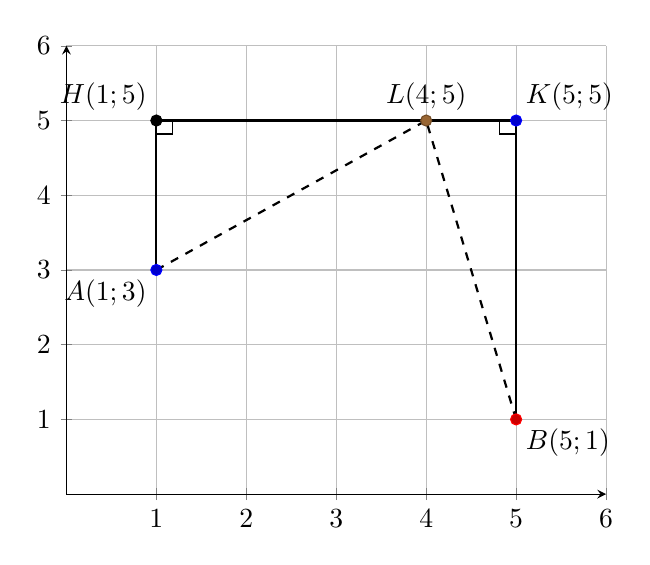
\begin{tikzpicture}
					\begin{axis}[
							xmin=0, xmax=6, ymin=0, ymax=6,
							grid=major,
							axis lines=middle,
							xtick distance=1, ytick distance=1,
							clip=false
						]
						% points (ordonnées réduites d'une unité)
						\addplot+[only marks, mark=*, mark size=2pt] coordinates {(1,3)}; \node[anchor=north east] at (axis cs:1,3) {$A(1;3)$};
						\addplot+[only marks, mark=*, mark size=2pt] coordinates {(5,1)}; \node[anchor=north west] at (axis cs:5,1) {$B(5;1)$};
						\addplot+[only marks, mark=*, mark size=2pt] coordinates {(4,5)}; \node[anchor=south] at (axis cs:4,5) {$L(4;5)$};
						\addplot+[only marks, mark=*, mark size=2pt] coordinates {(1,5)}; \node[anchor=south east] at (axis cs:1,5) {$H(1;5)$};
						\addplot+[only marks, mark=*, mark size=2pt] coordinates {(5,5)}; \node[anchor=south west] at (axis cs:5,5) {$K(5;5)$};

						% segments pour A-H-L
						\draw[thick] (axis cs:1,3) -- (axis cs:1,5);
						\draw[thick] (axis cs:1,5) -- (axis cs:4,5);
						\draw[thick,dashed] (axis cs:1,3) -- (axis cs:4,5);

						% segments pour B-K-L
						\draw[thick] (axis cs:5,1) -- (axis cs:5,5);
						\draw[thick] (axis cs:5,5) -- (axis cs:4,5);
						\draw[thick,dashed] (axis cs:5,1) -- (axis cs:4,5);

						% marques d'angle droit (petits carrés)
						\draw (axis cs:1,5) -- ++(0.18,0) -- ++(0,-0.18) -- ++(-0.18,0);
						\draw (axis cs:5,5) -- ++(-0.18,0) -- ++(0,-0.18) -- ++(0.18,0);

					\end{axis}
				\end{tikzpicture}

				\item Le triangle $AHL$ est rectangle en $H$ de côtés~:
				$$
					AH=|5-3|=2,\qquad HL=|4-1|=3.
				$$
				$$
					AL=\sqrt{AH^2+HL^2}=\sqrt{4+9}=\sqrt{13}.
				$$
				\item Le triangle $BKL$ est rectangle en $K$ de côtés~:
				$$
					BK=|5-1|=4,\qquad KL=|5-4|=1.
				$$
				$$
					BL=\sqrt{BK^2+KL^2}=\sqrt{16+1}=\sqrt{17}.
				$$
				\item Conclusion : $\sqrt{13}<\sqrt{17}\Rightarrow AL<BL$. Luc doit choisir la fontaine \textbf{A}.
			\end{MADenumerate}
		\end{multicols}
